%!TEX root = ../thesis.tex
%*******************************************************************************
%****************************** Second Chapter *********************************
%*******************************************************************************

\chapter{Continuous model} \label{ch:2}

\ifpdf
    \graphicspath{{Chapter2/Figs/Raster/}{Chapter2/Figs/PDF/}{Chapter2/Figs/}}
\else
    \graphicspath{{Chapter2/Figs/Vector/}{Chapter2/Figs/}}
\fi

Sheets of \textit{C. flexa}, despite being discretely made up of individual cells, appear to take on curvature when looked at as a whole. 
In an effort to develop an analytically tractable model for sheets consisting of many cells and avoid building a detailed network topology, I approximate here sheets of \textit{C. flexa} using continuous functions.

I begin by developing a one-dimensional filament model with inversion dynamics, which demonstrates that azimuthal stretching is key to understanding the flipping process observed in \citet{brunet2019}. 
I proceed to describe a method for approximating sheets of \textit{C. flexa} with two-dimensional surfaces and relate the collar-opening angle $\phi$ and collar-collar contact angle $\psi$ to surface curvature. 
I write an expression for the sheet energy but find that it yields no tractable shape equation.

\section{One-dimensional model} \label{sec:c_1d}

\begin{figure}[htbp]
	\centering
	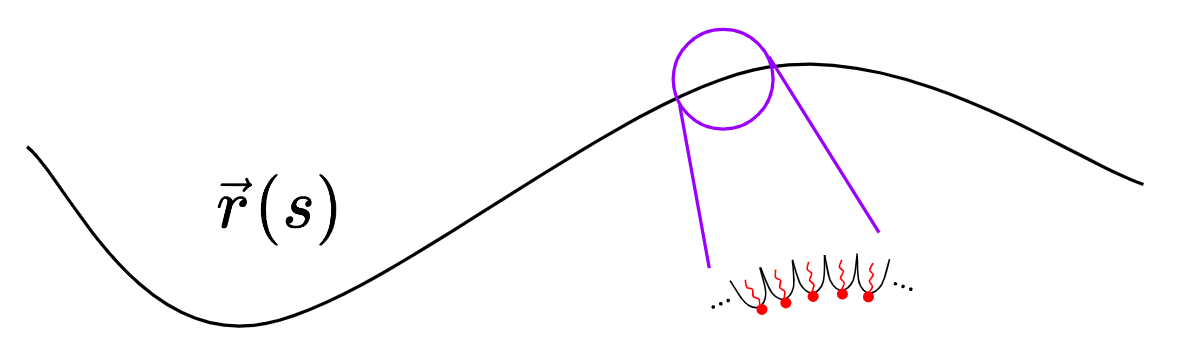
\includegraphics[width=\textwidth]{chain.png}
	\caption{Filament model of \textit{C. flexa} colonies}
	\label{fig:chain}
\end{figure}

To build intuition on the mechanics of \textit{C. flexa} inversion, consider a chain of cells connected by their collar filaments like beads on a string (\cref{fig:chain}). 
Supposing there are sufficiently many cells that the length contributed to the chain of cells by a single cell is small relative to the total length, we approximate the filament with a continuous function $\vec{r}(s, t)$ parameterised by arclength $s$ and changing in time $t$.
If the filament has preferred curvature $\kappa_0$, then the bending energy functional $\e$ is given by 

\begin{align*}
    \e[\vec{r}(s, t)] &= \frac{1}{2} a \int (\kappa - \kappa_0)^2 ds, 
\end{align*}
\noindent where the curvature $\kappa$ is deduced from $\vec{r}(s, t)$ and $a$ is the bending modulus. 

If the filament is short relative to the characteristic bending length scale, we express the problem in the Monge representation by writing $\vec{r}(s, t) = (x, h(x, t))$ for a height function $h(x, t)$, where $|h_x|$ is small.\footnote{Here, I use subscripts to denote partial derivatives: $h_x = \partial h / \partial x$. A number denotes several partial derivatives: $h_{3x} = \partial^3 h / \partial x^3$.} 
The resulting energy is written in terms of the prescribed (signed) curvature $H_0$, 
\begin{align}
    \e[\vec{h}(x, t)] &= \frac{1}{2} a \int_0^L (h_{xx} - H_0)^2 dx. \label{eq:energy}
\end{align}

Since the cells in this beads-on-a-chain description consist of large spheres connected by thin filaments, we postulate that the filament experiences isotropic drag with coefficient $\zeta$ in a viscous medium.
As a result, we describe the dynamics with a functional derivative of the energy with respect to the changing height,

\begin{align}
    \zeta \vec{r}_t &= -\frac{\delta \e}{\delta \vec{r}} \nonumber \\
    \zeta h_t &= -\frac{\delta \e}{\delta h}. \label{eq:eom} 
\end{align}
Taking the functional derivative of equation \ref{eq:energy}, we find the energy change
\begin{align}
    \delta \e &= \left. a(h_{xx} - H_0)\delta h_x \right|_0^L - \left. ah_{3x} \delta h \right|_0^L + a \int h_{4x} \delta h dx \label{eq:func_deriv} 
\end{align}
in terms of the boundary conditions of $h$.

For free boundary conditions (force- and torque-free edges) $h_{xx}(0, t) = 0, h_{xx}(L, t) = 0$ and $h_{3x}(0, t) = 0, h_{3x}(L, t) = 0$, the boundary terms in equation \ref{eq:func_deriv} vanish and we are left with the equation of motion 
\begin{align}
    \zeta h_t &= -a h_{4x}. \label{eq:eom_mange}
\end{align}

Equation \ref{eq:eom_mange} is nondimensionalised by re-expressing $x$ as $x/L$ and $t$ as $t / (\frac{\zeta L^4}{a})$ (the labels $x, t, h, H_0$ are left unchanged for readability) to derive $h_t = -h_{4x}$ with boundary conditions $h_{xx}(0, 1) = 0 = h_{3x}(0, 1)$. 
It is clear that the ground state of equation \ref{eq:energy} is given by a quadratic height function with quadratic term $\frac{1}{2}H_0x^2$. 
Let $h_*(x) = -\frac{1}{2} H_0(x-\frac{1}{2})^2 + \frac{1}{8}H_0$ be one such ground state, and suppose $h(x, 0) = -h_*(x)$. Note that the filament in $h(x, 0)$ is not in the ground state since the curvature is given by $-H_0$. 

The dynamics of the displacement $g(x, t) = h(x, t) - h_*(x)$ is given by $g_t = g_{4x}$. 
If $g(x, t) = e^{-\sigma t} f(x)$ for some $f(x)$ and eigenvalue $\sigma$, we obtain the ordinary boundary value problem 

\begin{align}
    \frac{d^4f}{dx^4} &= \sigma f & \begin{cases} f''(0, 1) = 0 \\ f'''(0, 1) = 0. \end{cases} \label{eq:bvp}
\end{align}

It is clear that the general solution of $f$ is $A \sin kx + B \cos kx + D \sinh kx + E \cosh kx$ \citep{landau1986}. 
As in \citet{wiggins1998}, the derivatives $f''(0) = f'''(0) = 0$ give $A = D, B = E$. 
Moreover, the eigenvalues $\sigma = k^4$ are given by the sequence of solutions $k_n$ to 

\begin{align}
    \cos k - \frac{1}{\cosh k} &= 0. \label{eq:roots}
\end{align}

Equation \ref{eq:roots} is plotted in Figure \ref{subfig:roots} along with the positions of the solutions $k_n$ as solved numerically. 
The solution $k_0 = 0$ is omitted because it contributes a constant term to $h(x, t)$ that does not evolve in time. 
The eigenfunctions $w_n(x)$ with eigenvalues $k_n^4$ are normalized on the interval $[0,1]$ numerically, and the ratio $A/B$ is given by $(\sinh k - \sin k) / (\cosh k - \cos k)$. 
The first five eigenfunctions are shown in Figure \ref{subfig:efuncs}. 

\begin{figure}[tbhp]
    \centering
    \begin{subfigure}[b]{0.48\textwidth}
        \centering
        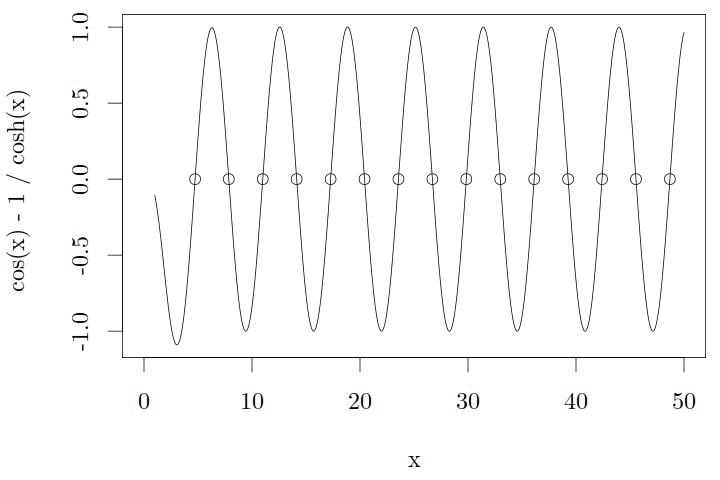
\includegraphics[width=\textwidth]{eq_roots.png}
        \caption{Equation \ref{eq:roots} and its solutions.}
        \label{subfig:roots}
    \end{subfigure}
    ~
    \begin{subfigure}[b]{0.48\textwidth}
        \centering
        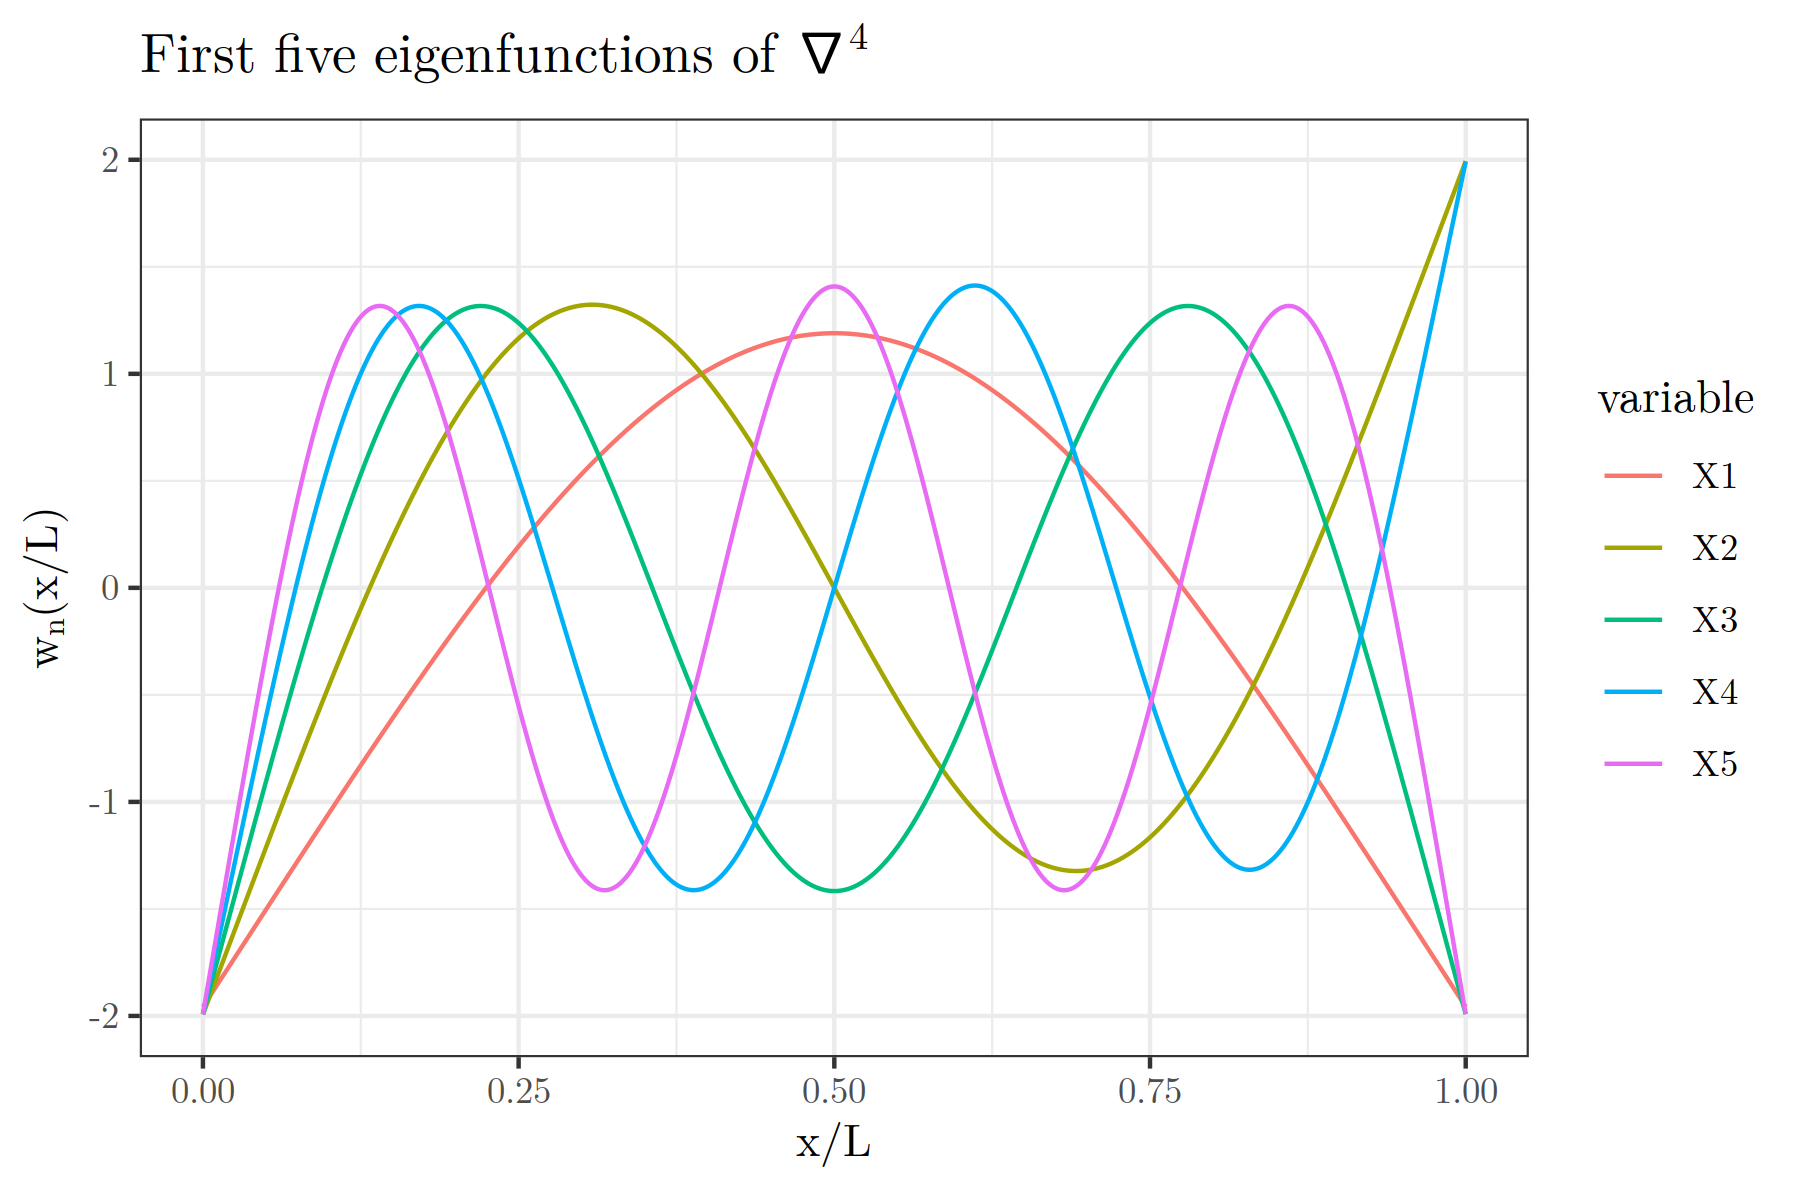
\includegraphics[width=\textwidth]{efuncs.png}
        \caption{The first five eigenfunctions $f_n$ of boundary value problem \ref{eq:bvp}.}
        \label{subfig:efuncs}
    \end{subfigure}
    \caption[Solutions to the biharmonic equation for a one-dimensional filament model]{Solving the boundary value problem in equation \ref{eq:bvp}}
    \label{fig:bvp_sol}
\end{figure}

Letting $f(x) = \sum_{n=1}^\infty a_n f_n(x)$, we get that $a_n = \int_0^1 g(x, 0) f_n(x)dx$, and the complete dynamics of the height function are given by 
\begin{align}
    h(x, t) &= h_*(x) + g(x) = h_*(x) + \sum_{n=1}^\infty a_n e^{k_n^4 t} f_n(x). \label{eq:sol}
\end{align}
\noindent In practice, only the solutions $k_n$ to equation \ref{eq:roots} shown in Figure \ref{subfig:roots} are used, since the approximation to $h(x, 0)$ is close and higher $k_n$ result in precision errors when calculating $\cosh kx$ and $\sinh kx$ (as in \citet{wiggins1998}). 

For the initial conditions given previously, the time evolution of $h(x, t)$ is shown in Figure \ref{fig:shapes}. 
We can observe that inversion occurs much more rapidly than the timescale defined by the fluid and system properties, which results from exponential decay with eigenvalues of $k_n^4$ in \cref{eq:sol}.
Moreover, we only weakly see a \textit{rolling over} effect observed at the edges of large inverting sheets \citep{brunet2019}, where a wave of changing curvature propagates from the edge of the sheet towards the centre.
Experimentally, the effect is more pronounced and occurs at the initiation of the transition.

Two limitations of this model stand out.
The first is the localised viscous drag assumed in \cref{eq:eom}, which allows a much faster inversion than would be allowed with nonlocal drag.
Here and later in this work (\cref{subsec:grad_desc}), I make this assumption to make solving for the dynamics of the problem more tractable.
However, this choice neglects the flows generated by each part of the organism and the effects those flows have on the surrounding parts of the colony.
Localised drag is reasonable in the limit that cells are spaced distantly from each other, as if they were connected via infinitely long and infinitesimally thin filaments.
Certainly this is not the case for \textit{C. flexa} colonies, where cell bodies can be spaced so closely as to press against each other.
The impact of the assumption I make here is somewhat ameliorated by the fact that resting flagella-in colonies sediment to the ground \citep{brunet2019}, though we generally do not know the extent to which drag due to nonlocal flow affects \textit{C. flexa} inversion and shape.
% Using Stokes' law $\zeta = 6 \pi \mu R$ for dynamic viscosity $\mu$ (about $\SI{1}{\kilo\gram\per\meter\per\sec}$) \citep{stokes1851} and cell radius $R\approx \SI{1e-6}{\meter}$ \citep{brunet2019}, a chain of 100 cells each contributing $\SI{5e-6}{\meter}$ length would require energy constant about 
% \mynote{finish the above. compare to bending modulus of flagella or microtubule or somethin} 

The second limitation is that the model used above does not penalise compression or stretching of the whole chain of cells, while stiffness in the collar would prevent the colony from changing in length\footnote{As a surface, area.} freely.
In particular, this is a consequence of the Monge representation used in \cref{eq:energy}.
Since a goal of this model is to capture sheet boundaries rolling over to initiate the transition, and this occurs slowly experimentally compared to the rapidly propagating wave of inversion afterwards, I chose to develop the model more to address this latter limitation.
The slow initiation of inversion for large sheets suggests that a mechanical barrier, rather than a dynamic one caused by interactions with the surround fluid, is responsible for the characteristic dynamics observed.
To address this, we find that compression and extension, especially in the azimuthal direction, are essential to understand the sheets' bistable nature.

\begin{figure}[bthp]
    \centering
    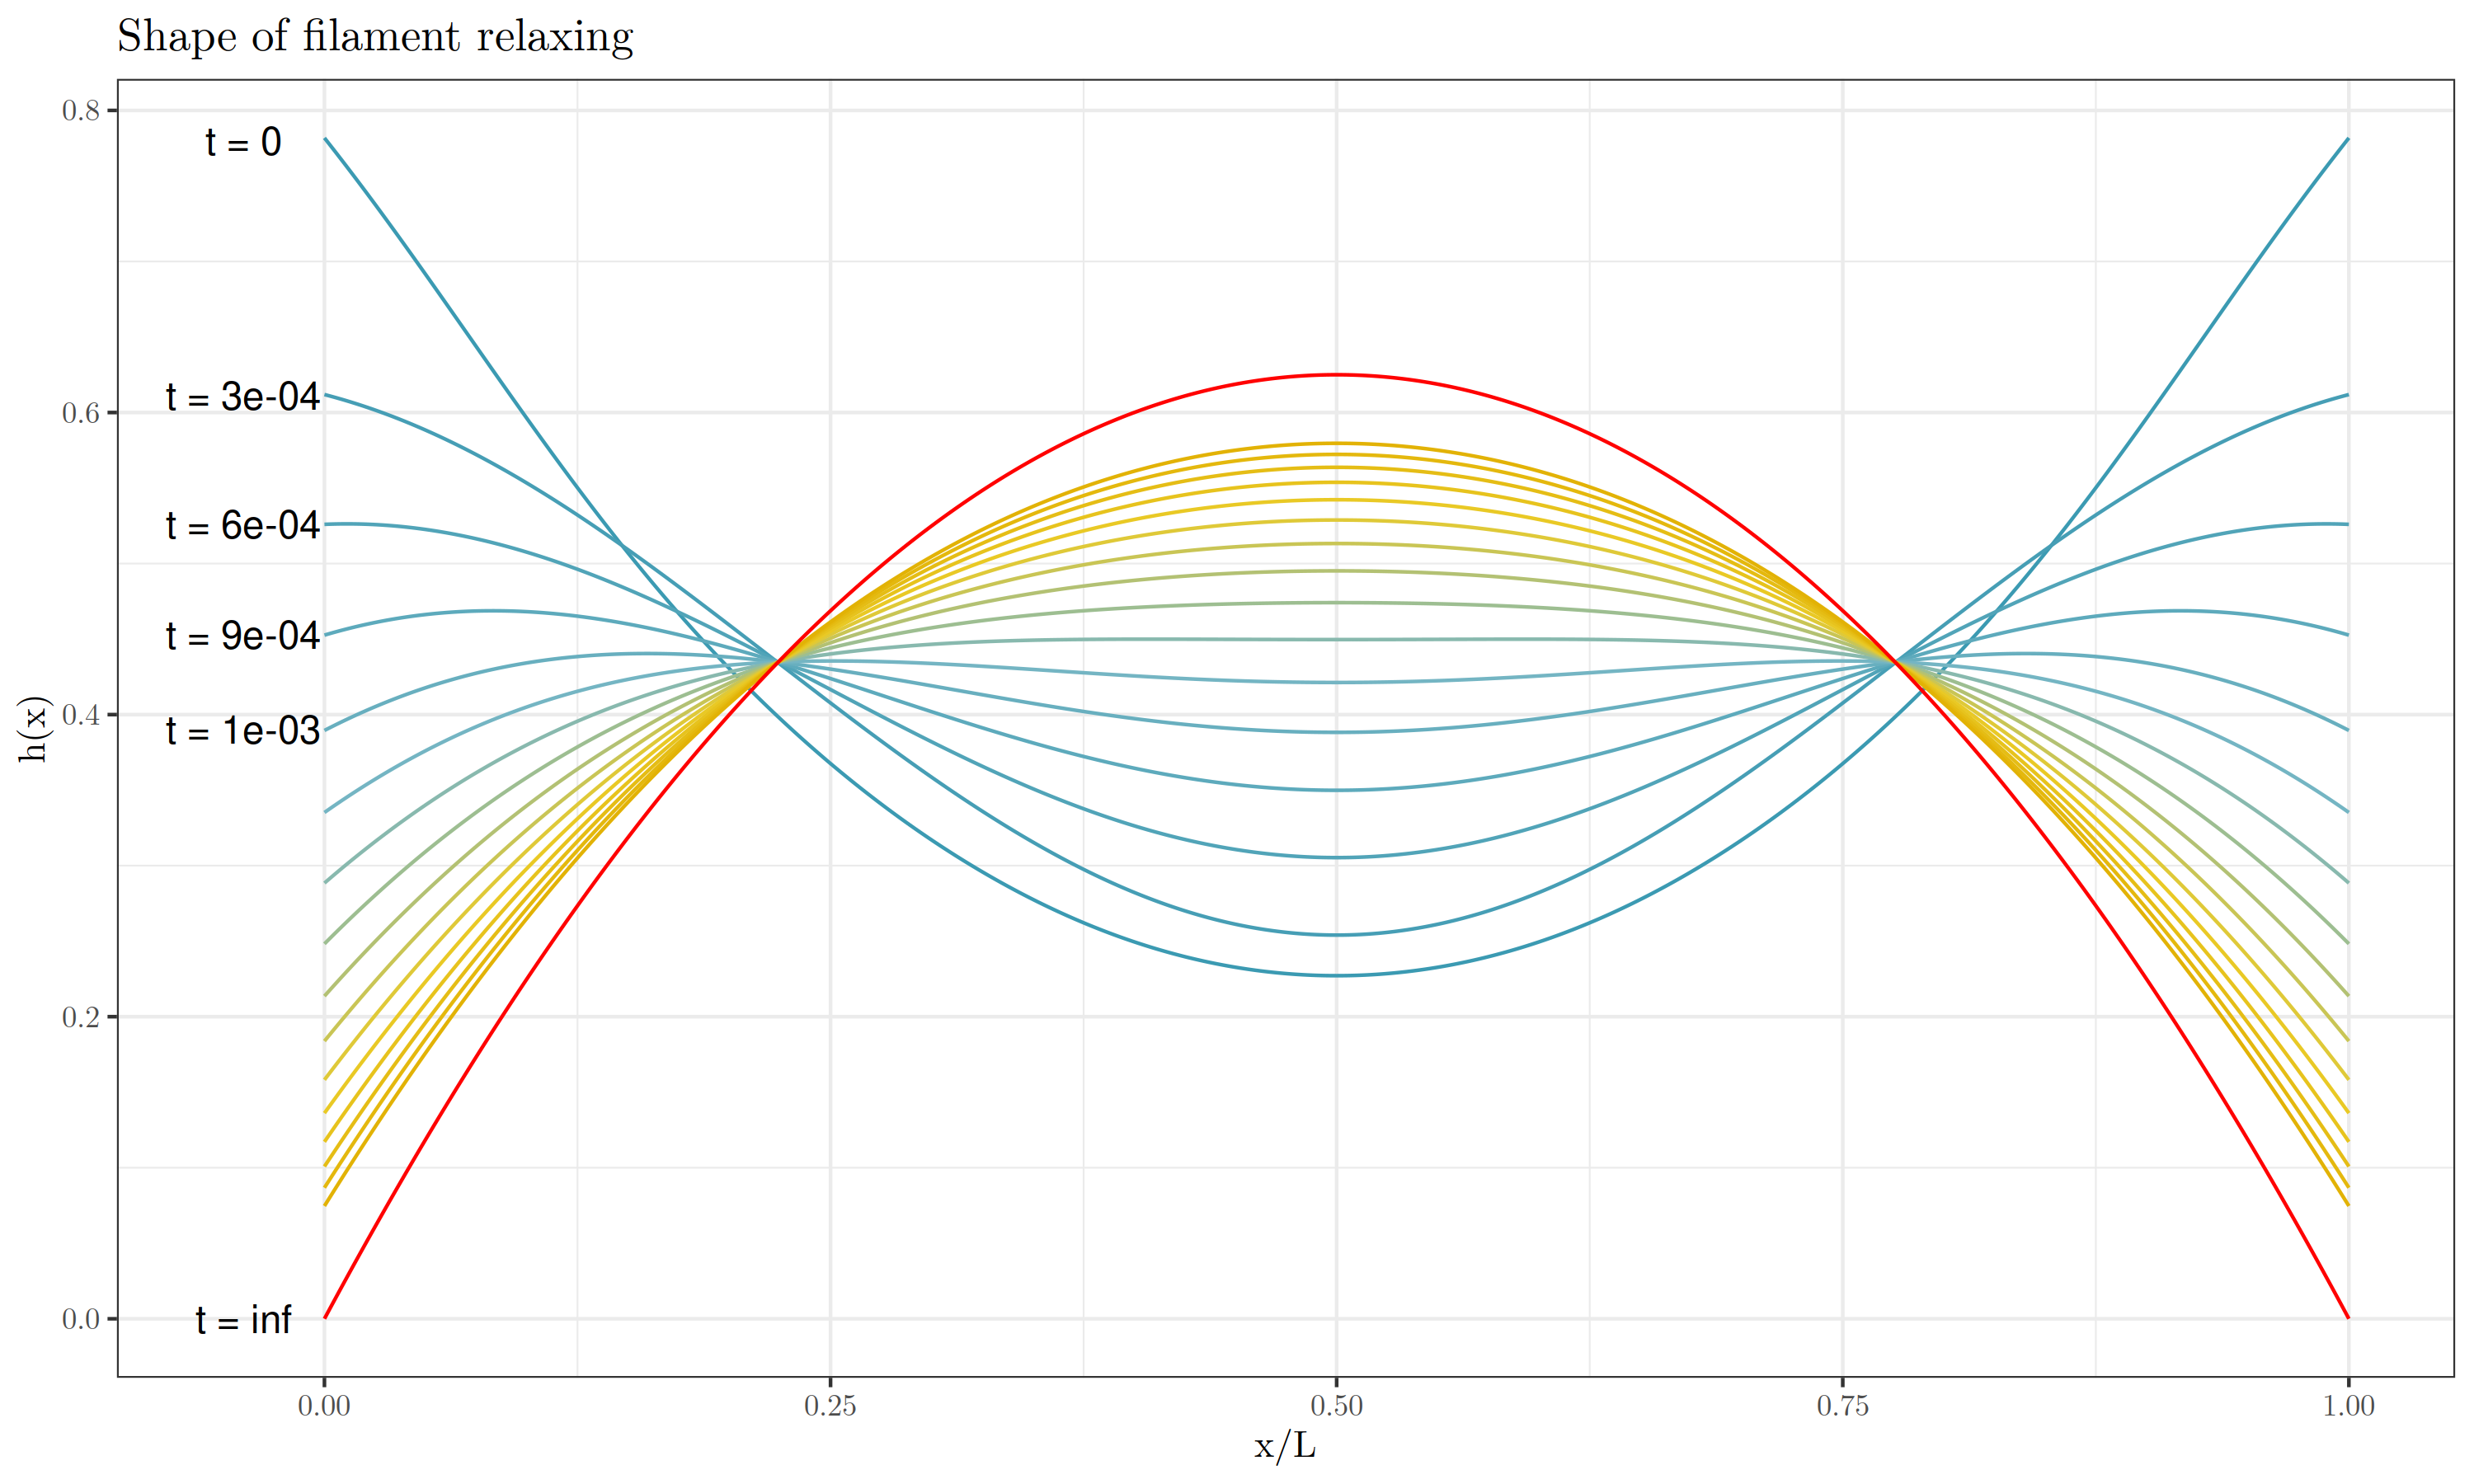
\includegraphics[width=\textwidth]{shapes.png}
    \caption[Dynamics of a one-dimensional filament model]{Time evolution of a one-dimensional filament which switches prescribed curvature sign instantaneously. Time and length are given in dimensionless units defined by the length $L$, bending modulus $k$, and drag coefficient $\zeta$. The time unlabeled time intervals continue sequentially in intervals of $\Delta t = \num{3e-4}$.}
    \label{fig:shapes}
\end{figure}

\section{Surface approximation} \label{sec:surface_approx}

The simplified dynamics that we get from the Monge representation lack energetic costs from the compression and extension that come with deforming a two dimensional surface. 
Here, I evaluate two continuous approaches to describing the sheet as a continuous surface that approximates the positions of collar-collar interfaces.
Since bending and stretching are coupled in \textit{C. flexa} sheets, I write a single energy function that encompasses both.

The resulting energy function is found to be too challenging to approach analytically and motivates \cref{ch:3} to describe the \textit{C. flexa} sheet as a discrete system.

\subsection{$H$ and collar connection angle} \label{subsec:h_phi}

\nomenclature[g-mn]{$\mu,\nu$}{Indices for a surface. $\mu,\nu \in \{1, 2\}$}
\nomenclature[a-g]{$g_{\mu\nu}$}{First fundamental form of a surface}
\nomenclature[a-k]{$K_{\mu\nu}$}{Second fundamental form of a surface}
\nomenclature[a-H]{$H$}{Mean curvature of a surface, the mean of the two principal curvature $g_{\mu\nu}K^{\mu\nu}/2$. Preferred mean curvature (constant) is denoted $H_0$}
\nomenclature[a-K]{$K$}{Gaussian curvature of a surface, the determinant of the second fundamental form $\det K_\mu^\nu$}

Before tackling the continuous sheet problem, it is worth describing the two degrees of freedom that our collar connections afford. 
The collar makes an angle $\phi$ between the vector pointing directly out of the cell and the vector between the cell and its collar boundary with the next cell. 
Additionally, there is an angle between the collars of two adjacent cells $\psi$. 
The latter results in the sheet's curvature. 
Hence, the goal is to relate the angles to the mean curvature $H$ or preferred curvature $H_0$.

\mynote{Discuss why we need a collar angle $\psi$ despite \citet{brunet2019} and other sources just talking about $\phi$. This has to do with the straight-collar approximation that I use, where the collar shape and curvature + clamped boundary condition of the meeting collars is distilled into two angles}

\begin{figure}[htbp]
    \centering
    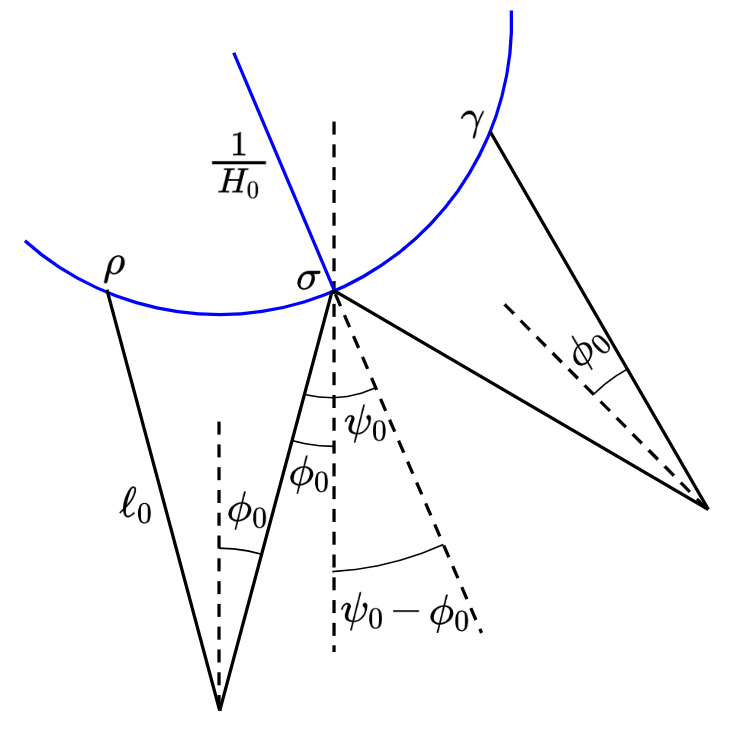
\includegraphics[width=0.5\textwidth]{hpsi.png}
    \caption[Geometry of sheet curvature]{Geometry for relating collar boundary angle $\psi$ to curvature $H$. The diagram represents a cross section in the plane formed by two neighbouring cells' bodies and the middle of the line along which their collars make contact. Cell bodies are represented by points at the intersections of black lines with bisecting angle $\phi_0$, and collars (black lines) make contact with neighbouring cells' collars at points $\rho$, $\sigma$, and $\gamma$. The non-physical blue arc represents a surface describing the collar-collar interfaces, where the radius of the circle is shown with a blue line of length $1/H_0$. The figure is not drawn to scale; roughly, $1/H_0 \sim \SI{50}{\per\micro\meter}$, $\ell_0 \sim \SI{10}{\micro\meter}$, and cell bodies (not pictured) have diameter about $\SI{4}{\micro\meter}$. (\Cref{ch:1})}
    \label{fig:hpsi}
\end{figure}

Consider two neighboring cells with collar boundaries $\rho$, $\sigma$, and $\gamma$, as shown in Figure \ref{fig:hpsi}. 
We seek to relate the preferred sheet curvature $H_0$ of units inverse length to the angles $\phi_0$ and $\psi_0$, the preferred angles that $\phi$ and $\psi$ take, and the preferred collar length $\ell_0$ with units of length.
I define a radius of curvature by the circle that passes through the three collar boundaries. 
Setting $\bm{x_\rho} = 2\ell\sin\phi_0(-1, 0)$, $\bm{x_\sigma} = (0,0)$, and $\bm{x_\gamma} = 2\ell\sin\phi_0 (\sin(\psi_0 - \phi_0), \cos(\psi_0-\phi_0))$, we solve for the circle's centre's coordinates 

\begin{align*}
    (x_\circ, y_\circ) &= \ell \sin\phi_0\left(-1, \frac{1+\cos2(\psi_0 - \phi_0)}{\sin2(\psi_0 - \phi_0)} \right)
\end{align*}

\noindent to get the inverse radius of curvature 

\begin{align}
    H_0 = \frac{1}{\sqrt{x_\circ^2 + y_\circ^2}} &= \frac{\sin(\psi_0 - \phi_0)}{\ell \sin\phi_0}. \label{eq:h0}
\end{align}

This has a simple interpretation in that if $\psi_0 > \phi_0$, $H_0 > 0$ (as drawn in Figure \ref{fig:hpsi}). On the other hand, $\psi_0 < \phi_0$ implies $H_0 < 0$, or the sheet is concave on the cell body side. 

Alternatively, we solve for $\psi_0$ as a function of $H_0$,

\begin{align}
    \psi_0 &= \phi_0 + \arcsin \left( H_0 \ell \sin \phi_0 \right). \label{eq:h0_psi}
\end{align}

As I find later in equation \ref{eq:hlb}, the curvature of the sheet in any given direction is greater than or equal to $-1/\ell$ (cell bodies and collars cannot go through each other). 
This lower bound corresponds in \ref{eq:h0_psi} to $\psi_0 = 0$, as expected when cell bodies are pressing tightly against each other (Figure \ref{fig:maxcurv}).

\subsection{Problem statement} \label{subsec:problem}

\citet{powers2010} shows that for an energy density $\e$ written in terms of the first and second fundamental forms $g_{\alpha\beta}$ and $K_{\alpha\beta}$, there is an expression for the stress tensor $\bm{F}^\alpha$ 

\begin{align}
    \bm{F}^\alpha &= \left(T^{\alpha\beta} + \e^{\alpha\gamma}K_\gamma^\beta \right)\bm{t}_\beta - (\nabla_\beta \e^{\alpha\beta})\hat{\bm{n}}, \label{eq:stress}
\end{align}

\noindent where summation over repeated indices is implied. Here, $K_\gamma^\beta = K_{\gamma \delta}g^{\delta \beta}$, $\bm{t}_\beta = \partial_\beta \bm{r}$, and 

\begin{align*}
    T^{\alpha\beta} &= g^{\alpha\beta} \e + 2 \frac{\partial \e}{\partial g_{\alpha\beta}} = \frac{2}{\sqrt{g}} \frac{\partial}{\partial g_{\alpha\beta}} \left(\sqrt{g}\e \right) \\
    \e^{\alpha\beta} &= \frac{\partial \e}{\partial K_{\alpha\beta}}
\end{align*}

\noindent with $g = \det{g_{\alpha\beta}}$.

Since the force $\bm{f}$ acting on a surface point is given by the covariant divergence of the stress $\nabla_\alpha \bm{F}^\alpha$, the problem is effectively solved once we decide on an appropriate energy density. 
I discuss two choices: one which introduces the energy density with separate bending and stretching energies from continuum mechanics and another developed by studying the geometry specific to \textit{C. flexa} cells.
\citet{brunet2019} showed that the angle formed by the \textit{C. flexa} collars changes when individual cells are triggered for inversion. 
It would appear reasonable then to suggest that preferred sheet curvature is prescribed by changing the preferred angle of the collar $\phi_0$ and impose an energetic cost based on the amount that the collar angle $\phi(\theta)$ differs around the collar in $\theta$: $\e \sim \int (\phi(\theta) - \phi_0)^2 d\theta$.

\subsection{Continuum surface mechanics approach} \label{subsec:cts}

I begin by describing the \textit{C. flexa} sheet as a thin plate with large deflections to define an energy density in terms of the strain tensor and displacement.
The displacement of a surface defined in the $xy$-plane can be described with a displacement vector function $\bm{u}(\bm{r})$ and deflection function $\zeta(\bm{r})$ so that $(x, y, 0)$ is mapped to $(x + u_x, y + u_y, \zeta)$ \citep{landau1986}.
Using the chain rule, we see that an infinitesimal length squared $ds^2$ on the surface $dx^2 + dy^2$ becomes 
\begin{align*}
	d{s'}^2 &= (dx + du_x)^2 + (dy + du_y)^2 + d\zeta^2 \\
	&= \left(dx + \frac{\partial u_x}{\partial x} dx\right)+ \left(dy + \frac{\partial u_y}{\partial y} \right)^2 + \left(\frac{\partial\zeta}{\partial x} + \frac{\partial\zeta}{\partial y} \right)^2 \\
	&= \delta_{ij} dx_i dx_j + \left(\frac{\partial u_i}{\partial x_j} + \frac{\partial u_j}{\partial x_i} + \frac{\partial \zeta}{\partial x_i} \frac{\partial \zeta}{\partial x_j}\right) dx_i dx_j \\
	&= (\delta_{ij} + u_{ij}) dx_i dx_j,
\end{align*}
where $i,j$ index over $1$ and $2$. The strain tensor $u_{ij}$, which describes infinitesimal displacement, is typically used to define a quadratic energy 
\begin{align}
	\e_s &= \frac{1}{2} \int_S \left( \sum_{i,j}2\mu u_{ij}^2 + \lambda u_{kk} \right) d^2r \label{eq:stretch}
\end{align}
as an infinitesimal form of Hooke's law \citep{landau1986}. 

The bending energy of membranes is often prescribed to be the Helfrich bending energy \citep{helfrich1973},
\begin{align}
	\e_b &= \int_S \left[ \frac{\kappa}{2} (2H - 2H_0)^2 + \kappa_G K \right] d^2r. \label{eq:helfrich}	
\end{align}
\noindent Here $H=1/2 (g_{\mu\nu}K^{\mu\nu})$ is the mean curvature of the sheet given by $\bm{u}$ and $\zeta$ and $K = \det K_\mu^\nu$. 
The model \cref{eq:helfrich} is commonly found in studies of fluid membrane curvature, particularly for lipid bilayers or micelles formed using surfactants \citep{andelman1994,seifert1997}.
Since \textit{C. flexa} sheets do not form closed surfaces, any shape equation from \cref{eq:helfrich} must come with appropriate boundary conditions. 
\citet{tu2003} derived a general equilibrium solution to \cref{eq:helfrich} with boundary, as well as the simplified axisymmetric case, by taking the functional variation of \cref{eq:helfrich} with respect to the surface position.

\citet{seung1988} derived the equilibrium solution to the simultaneous stretching and bending problem in the limit of small $|\nabla \zeta|$, analogous to the approximation used in \cref{sec:c_1d}.
The resulting equations are too difficult to solve \citep{landau1986}, but the authors find that Gaussian curvature effectively cancels stress due to disclinations and dislocations, or topological defects in the underlying surface crystal structure \citep{sachdev1984}.
The shape equations derived from functional variations of \cref{eq:stretch,eq:helfrich} may be solved in the inextensional limit that $\mu,\lambda \to\infty$ and show that topological defects produce buckling.

Since we know well that collars may vary in end-to-end length, the limit solution to the resulting shape equations is unrealistic and we would resort to treating the problem numerically.
Additionally, as in \cref{subsec:h_phi}, sheet bending and collar angle (hence, sheet stretching) are coupled. 
Due to this coupling, I aimed to write a combined energy density for use in \cref{eq:stress} with the goal of deriving a more manageable solution.
\mynote{qualify that collars may vary in length}

\subsection{Connecting continuous surface with individual cell mechanics}

Following cues from the experimental descriptions of \textit{C. flexa} collars, I sought to write an energy density in terms of the collar angle $\phi$. 
Since $\phi$ may vary around a cell at some position on the sheet, I write $\phi(\theta)$ as a function of angle $\theta$ varying from $0$ to $2\pi$ around the cell.
Then the energy density is written proportionally to the integral of squared deviation of $\phi$ from a reference collar angle $\phi_0$,
\begin{align}
	\e &= \int_0^{2\pi} (\phi(\theta) - \phi_0)^2 d\theta. \label{eq:phi_int}
\end{align}
I proceed by deriving the relationship between $\phi(\theta)$ and the second fundamental form $K_{\mu\nu}$ which describes the sheet curvature.

For any point on a smooth surface, we could find an orthonormal basis of eigenvectors $\bm{e}_1, \bm{e}_2$ in the tangent space that diagonalises $K_\mu^\nu$. 
In terms of a small displacement vector $\bm{\Delta \xi}$ written in this basis, the change in height $\Delta h$ with respect to the tangent plane and its normal is given by $K_{\mu\nu}\Delta\xi^\mu\Delta\xi^\nu$ \citep{powers2010}.

If the cell has an optimal collar angle $\phi_0$ and corresponding optimal curvature $K_{0\mu\nu}$, then the height of the collar will be $K_{0\mu\nu}\Delta\xi_0^\mu\Delta\xi_0^\nu$. 
The distance from the centreline of the cell (the norm of $\bm{\Delta\xi_0}$) is determined by $\phi_0$. The geometry is shown in Figure \ref{fig:geom}, where the collar length $\ell$ is kept fixed.

\begin{figure}[htbp]
    \centering
    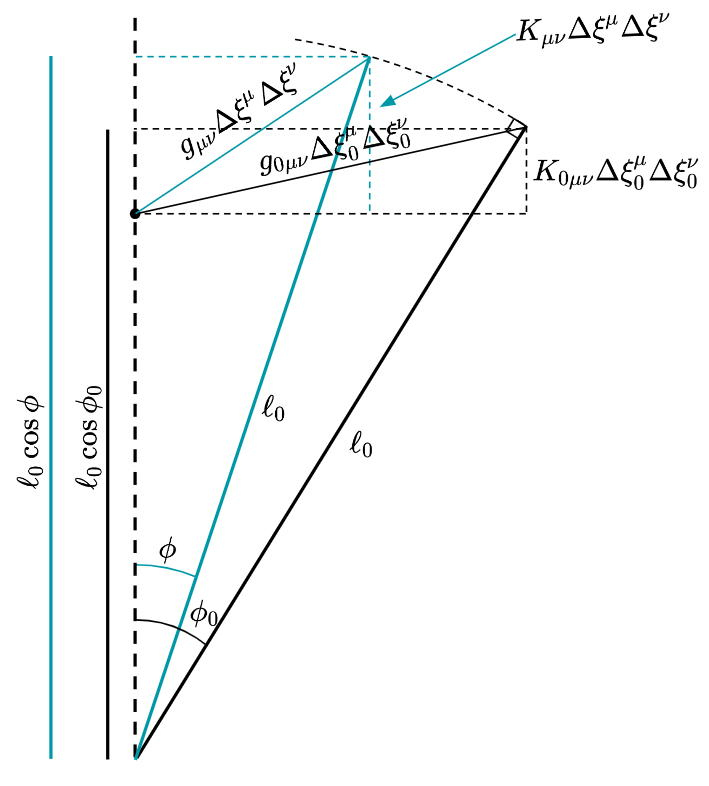
\includegraphics[width=0.75\textwidth]{geom.png}
    \caption[Geometry for continuous approximation of \textit{C. flexa} sheets]{Geometry of a single cell and collar with a continuous surface approximating the interactions between collars.}
    \label{fig:geom}
\end{figure}

\mynote{make these vectors here three dimensional}
If the cell has collar angle $\phi$ in direction $\theta$, we know the collar distance as $\bm{\Delta\xi} = \ell(\cos\phi, \sin\phi)$.\footnote{These calculations are temporarily done in the cell-collar plane, assuming that the collar extends only radially from the apicobasal axis. \Cref{fig:geom} is drawn showing geometry in this plane.} 
For a fixed collar length $\ell$, we know the difference in height between the ground state and deformed state is $\ell(\cos\phi - \cos\phi_0)$. 
We can then relate the collar angle and sheet curvature by equating 

\begin{align}
    K_{\mu\nu}\Delta\xi^\mu\Delta\xi^\nu - K_{0\mu\nu}\Delta\xi_0^\mu\Delta\xi_0^\nu &= \ell(\cos\phi - \cos\phi_0). \label{eq:base}
\end{align}

The radius out from the center for the ground state is $\ell\sin\phi_0$ while for the deformed state it is $\ell\sin\phi$, so for $K_{011}=K_{022}=H_0$, we get

\begin{align*}
    K_{\mu\nu}\ell^2\sin^2\phi (\cos\theta, \sin\theta)^{\mu,\nu} - H_0 \ell^2\sin^2\phi_0 &= \ell(\cos\phi - \cos\phi_0) \\
    H_\theta \ell^2\sin^2\phi - H_0 \ell^2\sin^2\phi_0 &= \ell(\cos\phi - \cos\phi_0)
\end{align*}

\noindent where $H_\theta = K_{11}\cos^2\theta + K_{22}\sin^2\theta + 2K_{12}\sin\theta\cos\theta$ is the curvature of a line on the surface in direction $\theta$. 
We can cancel a factor of $\ell$, redefine units of length in terms of $\ell$ (such that $H_\theta$ is the ratio of $\ell$ with the radius of curvature in direction $\theta$), and express $\sin^2\phi$ in terms of $\cos\phi$ to get

\begin{align*}
    0 &= H_\theta \cos^2\phi + \cos\phi + (H_0\sin^2\phi_0 - \cos\phi_0 - H_\theta) \\
    \cos\phi &= \frac{-1 \pm \sqrt{1 + 4H_\theta (H_\theta + \cos\phi_0 - H_0\sin^2\phi_0)}}{2H_\theta}.
\end{align*}

If we take the collars to always have angle $0 \leq \phi \leq \pi/2$, we can constrain $0 \leq \cos\phi \leq 1$ to find the two inequalities 

\begin{align}
    H_\theta \geq H_0 \sin^2\phi_0 - \cos\phi_0 \label{eq:ineq1}\\
    1 \geq \cos\phi_0 - H_0 \sin^2\phi_0. \label{eq:ineq2}
\end{align}

\noindent The second inequality can be simplified to $H_0 \geq -(1+\cos\phi_0)^{-1}$. 
Combining the two inequalities yields 

\begin{align}
    H_\theta \geq -1. \label{eq:hlb}
\end{align}

\noindent Re-expressed with units, \cref{eq:hlb} expresses that $H_\theta \geq -1/\ell$, or that the radius of curvature can never be smaller than $\ell$ on the cells' side. 
Physically, we understand this to mean that cells are unable to push through each other (\cref{fig:maxcurv}).

\begin{figure}[hbtp]
    \centering
    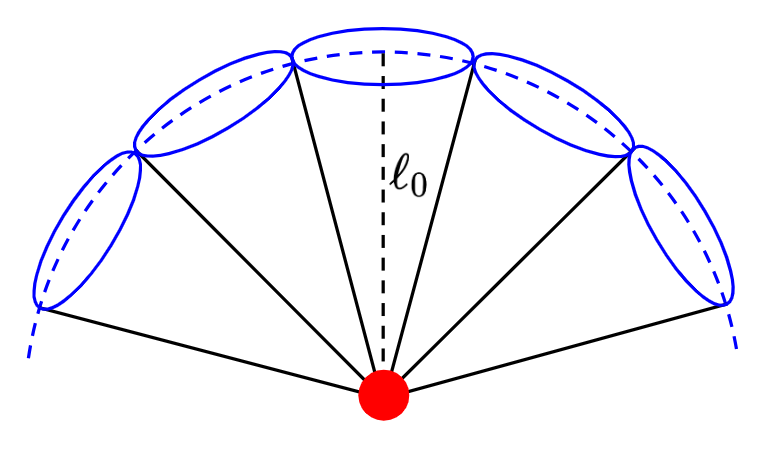
\includegraphics[width=0.5\textwidth]{arc.png}
    \caption[Bounded sheet curvature permitted in the continuous sheet description]{Maximum cell-side curvature is given by inequalities \ref{eq:ineq1}, \ref{eq:ineq2} to have radius $\ell$. This corresponds to every (point) cell bumping into each other.}
    \label{fig:maxcurv}
\end{figure}

\subsection{Writing the energy}

We want to write equation \ref{eq:base} in terms of $\phi-\phi_0$ to write down the energy. We can use a trigonometric identity to write

\begin{align}
    H_\theta \sin^2\phi - H_0 \sin^2\phi_0 &= -2 \sin \frac{\phi - \phi_0}{2} \sin\frac{\phi + \phi_0}{2}. \label{eq:preapprox}
\end{align}

\noindent If $\phi - \phi_0$ is small in magnitude, then 

\begin{align*}
    \sin\frac{\phi - \phi_0}{2} &\approx \frac{\phi - \phi_0}{2} \\
    \sin\frac{\phi + \phi_0}{2} = \sin\left(\phi_0 + \frac{\phi + \phi_0}{2} \right) &\approx \sin\phi_0 + \frac{\phi - \phi_0}{2} \cos\phi_0 \\
    \sin^2\phi = \sin^2\left(\phi_0 + (\phi - \phi_0) \right) &\approx \sin^2\phi_0 +(\phi - \phi_0)\sin2\phi_0.
\end{align*}

Using these approximations we rewrite equation \ref{eq:preapprox} to first order in $\phi - \phi_0$ as

\begin{align*}
    (H_\theta - H_0) \sin^2\phi_0 + H_\theta (\phi - \phi_0)\sin2\phi_0 &= -(\phi - \phi_0) \sin\phi_0 \\
    (H_\theta - H_0) \sin^2\phi_0 &= -(\phi-\phi_0) (H_\theta \sin2\phi_0 + \sin\phi_0) \\
    \frac{(H_\theta-H_0)^2 \sin^4\phi_0}{(H_\theta + \sin\phi_0 / \sin2\phi_0)^2 \sin^2 2\phi_0} &= (\phi - \phi_0)^2.
\end{align*}

To integrate this function in $\theta$ (\cref{eq:phi_int}, let $K_{11} = a$, $K_{22} = b$, $K_{12} = c$, $-H_0 = d$ and $\sin\phi_0/ \sin 2 \phi_0 = e$ for simplicity when we write

\begin{align}
    \int_{-\pi}^\pi (\phi - \phi_0)^2 d\theta &= \int_{-\pi}^\pi \frac{\left(a\cos^2\theta + b\sin^2\theta + 2c\sin\theta\cos\theta + d \right)^2}{\left(a\cos^2\theta + b\sin^2\theta + 2c\sin\theta\cos\theta + e \right)^2} d\theta. \label{eq:integral}
\end{align}

The integral in \cref{eq:integral} can be solved analytically and expressed in terms of $H$ and $K$ (Appendix \ref{apx:cts}), 

\begin{align}
    \int_{-\pi}^\pi (\phi - \phi_0)^2 d\theta &= \text{const.} + \text{const.} \frac{4 K + 2(d+3e)H + 2de + e^2}{(K + 2H + e^2)^{3/2}}. \label{eq:phi_int_complete}
\end{align}

Varying the energy density defined by \cref{eq:phi_int_complete} (from \cref{eq:phi_int}) is more challenging than the Helfrich membrane energy density (\cref{eq:helfrich}) since there is no term linear in $K$. 
As a result, the Gauss-Bonnet theorem $\int_S K d^2r = 2\pi n + \oint_{\partial S} K ds$ for an integer $n$ based on surface topology cannot be used to reduce the effects of Gaussian curvature to boundary conditions.

\subsection{Energy variation}

The energy density \cref{eq:phi_int_complete} can be varied directly or used in \cref{eq:stress} to solve forces on the sheet or the equilibrium shape equations.
While the functional variation is possible and not too challenging for the surface interior (Appendix \ref{apx:cts}), the resulting shape equation is clearly unapproachable in a simple way.
Since obtaining an approximate solution would require a numerical implementation, we are better suited to treat the sheet as the interactions between several discrete units.

\mynote{move this to the appendix apx:cts}
% Following subsection \ref{subsec:problem}, we just need to express our energy in terms of $K_{\mu\nu}$ and $g_{\mu\nu}$ to derive a force from it. We of course have that $H = (1/2) (K_{\mu\nu} g^{\mu\nu})$, which is easily differentiated with respect to $K_{\mu\nu}$ and $g_{\mu\nu}$. We can differentiate $K$ by re-expressing it with the identity $K^{\alpha\beta}K_{\alpha\beta} = 4H^2 - 2K$.\footnote{This comes from $4H^2 - 2K = (K^1_1 + K^2_2)^2 - 2(K^1_1K^2_2 - 2K^1_2) = (K^1_1)^2 + 2 K^1_2K^1_2 + (K^2_2)^2 = K^\alpha_\beta K_\alpha^\beta = K^{\alpha\beta}K_{\alpha\beta}$.} Then we have $K = (g^{\alpha\beta}K_{\alpha\beta})^2 - K_{\mu\nu}K_{\alpha\beta}g^{\mu\alpha}g^{\nu\beta}$.
